\documentclass[12pt, a4paper]{article}
\usepackage[T2A]{fontenc}
\usepackage[russian]{babel}
\usepackage[margin=0.6in]{geometry}
\usepackage{amssymb}
\usepackage{amsmath}
\usepackage{graphicx}
\usepackage{blindtext}
\usepackage[none]{hyphenat}
\usepackage[expansion=false]{microtype}
\emergencystretch=3em
\def\D{\mathbb}
\graphicspath{{images/}}

\title{Изследване на Операциите}
\author{Матей Захариев}
\date{}
\begin{document}
\maketitle

{\centering\section*{Информация за курса}}

Професор: Надя Златева;  2 контролни и 2 домашни, възможност за освобождаване от практика. Контролните не са задължителни. Първо писмено контролно на 19.12, второ - 10.01 на компютър. Писмен изпит: 25.01\\

{\centering\section*{08.10.2026}}
\subsection*{Изследване на операции(Operations research)}
Какво е \textbf{операция}? Имаме множество операции. Медицински, военни, екологични, производствени, т.н. Операция е определена последователност от действия с дефинирана цел.\\
Какво е \textbf{изследване}? Анализ на провеедените операции въз основа на научни методи - математика.\\
Сравнително млада дисциплина, възникнала по време на Втората Световна Война.\\
Ще разгледаме \textbf{задачата на организационното управление} чрез пример на промишлено производство на кофи и контейнери за боклук.\\
\begin{itemize}
\item \textbf{Цел.}\\
Това е какво опитваме да постигнем с нашата операция.\\
\textit{Правим кофи за боклук? Какви различни видове aaa имаме: метални кофи и кнетейнери и пластмасови контейнери. Всеки продукт изисква различни материали, нека използваме метал, пластмаса и гума. Всеки продукт има и пазарна цена. Такава задача може примерно да има следните \textbf{цели}: Максимизиране на печалбата(приходи); Минимизиране на загубите.}
\item \textbf{Постоянни}(константи).\\
Това са непроменливите фактори в нашата операция, които определят границите, в които работим и параметрите, върху които оптимизираме.\\
\textit{Вече споменахме няколко такива в този пример. Можем да дефинираме следните: използван материал за даден продукт, печалба на продукт, скалдиран материал, изисквания по договор, т.н. Те определят колко можем и трябва да произведем и как оптимизираме тяхното производство. Можем да ги подредим в следната таблица:}
\begin{center}
\begin{tabular}{|c||c|c|c|c|}
\hline
 & метал & пластмаса & гума & печалба\\\hline\hline
метална кофа & 5кг & 1кг & 0кг & 50 евро\\\hline
метален контейнър & 80кг & 2кг & 3кг & 300 евро\\\hline
пластмасов контейнър & 2кг & 30кг & 2кг & 200 евро\\\hline
склад & 5000 кг & 2000 кг & 300 кг&\\\hline
\end{tabular}
\end{center}

\item \textbf{Променливи.}\\
Фактори, които можем да променяме. Оптимизацията се извършва върху тези променливи и крайното решение е стойността на тези променливи за достигане на целта.\\
\textit{В дадения пример променливите са броя произведени кофи от всеки вид. Съответно можем да сведем задачата до максимизиране на следната функция:}
\[f(x_1,x_2,x_3)=50x_1 + 300x_2+200x_3\]
\textit{Теоритично имаме безкраен максимум, но постоянните ни поставят лимит от допустими стойности. Можем да ги опишем като система:}
\[
\begin{cases} 
5x_1+80x_2+3x_3\leq5000 \\ 
x_1+2x_2+30x_3\leq2000 \\
3x_2+2x_3\leq300 \\
x_1, x_2, x_3 \geq 0
\end{cases}
\]
\textit{Можем да имаме и други лимити, примерно долна граница по договор за произведени контейнери: $x_1 + x_2 \geq 100$}
\end{itemize}
\subsection*{Математическия модел}
Горният пример показва цялостния математически модел на една задача на линейно оптимиране(ЗЛО). В този модел имаме:
\begin{itemize}
\item \textbf{целева функция: f};
\item краен брой \textbf{променливи: $x_i; i = 1...k$};
\item \textbf{критерии} - целта(max или min) над функцията;
\item \textbf{ограничения} от вида $g_i(x_1, ... x_k) </>/= b_i$. 
\end{itemize}
Над линейното пространство ние работим с вектори(точки). Ограниченията ни определят \textbf{допустимото множество} и всяка точка от това множество наричаме \textbf{допустима стойност}. (Оптимално) \textbf{решение} на задачата е такава допустима точка, т.че. в нея целевата функция приема максимална (минимална) стойност измежду допустимото множество. \textbf{!!!Решението е вектор!!!} Стойността на целевата функция в оптималното решение се нарича оптимална стойност.
\subsection*{Етапи на изследване на операции}
\begin{enumerate}
	\item Описание на проблема (словесно).
	\item Моделиране.
	\item Решаваме задачата чрез модела.
	\item Проверка за адекватност на модела. (Ако не е адекватен, обратно към моделиране)
	\item Внедяване на решението
\end{enumerate}

{\centering\section*{15.10.2026}}

Ще разгледаме Следния пример за ЗЛО:\\
$
\left|
\begin{array}{l}
	max z(x) = 3x_1-2x_2\\
	x_1-2x_2\leq1\\
	4x_1+3x_2\leq15\\
	x_1+2x_2\geq-1\\
	x_2\geq0
\end{array}
\right.
$\\
Съответно можем да го решим геометрично чрез графика. Първо си построяваме правите определящи допустимото множество за да можем да го дефинираме. После чертаем нормалният вектор на целевата функция и разглеждаме в коя част проекцията на допустимото множество е максимална.
\begin{center}
	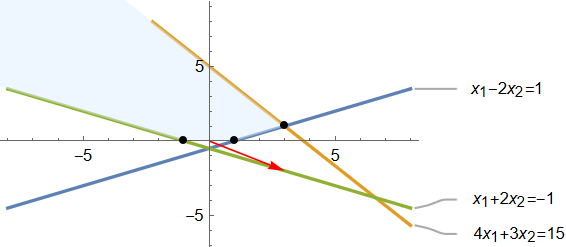
\includegraphics[scale=0.6]{graph2}
\end{center}
На графиката виждаме, че най-дясната точка има най-голяма проекция спрямо нормалният вектор. Съответно намираме нейните координати (3,1) и стойността на целевата функция в тях: 7.\\
Нека разгледаме втори пример със същото допустимо множество и целева функция $z(x) = 3x_1-6x_2$:
\begin{center}
	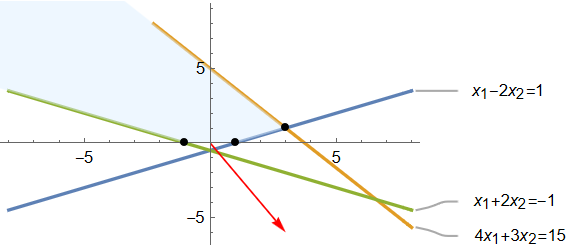
\includegraphics[scale=0.6]{graph1}
\end{center}
Защото нормалният вектор на втората права съвпада с този на целевата функция, те са перпендикулярни и цялата отсечка е оптимално решение. Записваме $x^*=(\lambda,\frac{\lambda-1}{2}), \lambda\in[1,3]$.\\

\subsection*{Канонична ЗЛО}
Всяка ЗЛО може да се представи в следния каноничен вид:\\
\begin{enumerate}
	\item Винаги търсим минимум на целевата функция. Ако задачата изисква максимум разглеждаме $max(z(x)) = -min(-z(x))$
	\item Всяка свободна променлива (за която нямаме $x_j\geq0$) се представя като разлика на две нови неотрицателни променливи: $x_j = x_j^+ - x_j^-$
	\item Всяко $b_j$ е положително. Постигаме като умножаваме по -1 където не е изпълнено.
	\item При условие $\sum_{j=1}^{n}a_ijx_j\leq b_j$ добавяме нова променлива за да допълним до равенство: $\sum_{j=1}^{n}a_ijx_j+x'= b_j$
	\item Аналогично като при горното, при $\geq$ изваждаме нова променлива.
\end{enumerate}
Нека трансформираме горния пример към каноничен вид:\\
\begin{enumerate}
	\item Търсим max, така че променяме и вече търсим $min z(x) = -3x_1 + 2x_2$
	\item Разделяме $x_1$ на две променливи: $x_1 = x_1^+ - x_1^-$ 
	\item Умножаваме третото неравенство по -1: $-x_1^+ +x_1^--2x_2=1$
	\item Добавяме $x_3$, $x_4$ и $x_5$ за всяко неравенство за да го превърнем в равенство.
\end{enumerate}
Каноничния вид е следния:\\
$
\left|
\begin{array}{l}
	min z(x) = -3x_1^+ +3x_1^- +2x_2\\
	x_1^+-x_1^--2x_2+x_3=1\\
	4x_1^+-4x_1^-+3x_2+x_4=15\\
	-x_1^++x_1^--2x_2+x_5=1\\
	x_j\geq0
\end{array}
\right.
$\\
В този вид можем да въведем матричен запис:
\[z(x)=c^Tx; A\in \D{R}^{mxn}; b\in\D{R}_+^m;\]
\[
\left|
\begin{array}{l}
	Ax=b\\
	x\geq\sigma
\end{array}
\right.
\]
А е матрица с пълен ранг. Ако вземем $B\in\D{R}^{mxm}$ подматрица на А тогава следното наричаме базисно решение: $\overline{x}=
\begin{bmatrix}
	B^{-1}b\\
	\sigma
\end{bmatrix}
$. Ако $\overline{x}\geq\sigma$, наричаме допустимо базисно решение. Ако $\overline{x}\in М$, където M е допустимото множество, тогава:\\
\begin{enumerate}
	\item $\overline{x}$ е връх на M;
	\item $\overline{x}$ е базисно допустимо решение;
	\item На положителните координати на $\overline{x}$ се съпоставят линейно независими стълбове на A.
\end{enumerate}

Ако $\overline{x}$ е връх на M и броя положителни координати е равен на броя уравнения, тогава $\overline{x}$ наричаме \textbf{неизроден връх} и има единствен базис B съставен от съответните стълбове на A. Ако $\overline{x}$ е връх на M и броя положителни координати е по-малък от броя уравнения, тогава $\overline{x}$ наричаме \textbf{изроден връх} и може да има повече от един базис B съставен от съответните стълбове на A допълнен до квадратна с друг линейно независим стълб от А.\\

{\centering\section*{22.10.26}}
Имаме три вида канонична задача:
\begin{enumerate}
	\item $M = \emptyset$. Нямаме решения, наричаме задачата несъвместима.
	\item $M \ne \emptyset$ и $z(x)$ е неограничана отдолу върху M, т.е. $\exists\{x_k\}_{k=0}^\infty$ т.че $z(x_k)=c^Tx_k\rightarrow\infty$ за $k\rightarrow\infty$. Наричаме задачата неограничена.
	\item $M \ne \emptyset$ и $z(x)$ е ограничена отдолу върхо M. Съществува оптимално решение. Наричаме задачата разрешима.
\end{enumerate}

\textbf{Деф.} Нека $x_1, x_2 \in \D{R}^n$. Изпъкнала комбинация на двата вектора се нарича всяка точка от вида $x=\lambda x_1 + (1-\lambda)x_2$ за $\lambda\in[0,1]$. $\lambda$ и $(1-\lambda)$ се наричат тегла. Ако $\lambda \in (0,1)$, то наричаме комбинацията истинска.\\

\textbf{Деф.} Едно множество C наричаме изпъкнало ако за всеки две точки $x_1, x_2 \in M$, всяка тяхна изпъкнала комбинация също принадлежи на C. По дефиниция празното множество и едноточковите множества са изпъкнали.\\

\textbf{Деф.} Точка $\overline{x}$ от изпъкнало множество C наричаме връх на C ако не може да се представи като истинска изпъкнала комбинация на две точки.\\

Примери: Кръг, правоъгълник, триъгълник, правилни многоъгълници включително вътрешността им са изпъкнали множества. Правоъгълникът има 4 върха, триъгълникът 3, кръгът безкрайно много - цялата обиколна окръжност се съости от върхове.\\

\textbf{Деф.} За множество от точки $\{x_k\}_{k=1}^n$, тяхна изпъкнала комбинация е точка от вида $x=\sum_{k=1}^n\lambda_kx_k$ за $\lambda_k \geq 0, \sum_{k=1}^n\lambda_k=1$\\

\textbf{Деф.} Изпъкнала обвивка на едно множество B дефинираме C - най-малкото множество, съдържащо всички изпъкнали комбинации на точки от B. $C = \{x = \sum_{k=1}^n\lambda_kx_k; \{x_k\}_{k=1}^n\subseteq B\}$\\

\textbf{Деф.} Симплекс с размерност k е изпъкнала обвивка на k+1 точки, където $x_1-x_0, ... x_k-x_0$ са линейно независими.\\
Пример: Триъгълникът и тетраедърът са симплекси, но правоъгълникът не е.\\

\textbf{Твърдение:} Крайно сечение на изпъкнали множества е изпъкнало множество.\\
\textbf{Доказателство:} Нека $x_1, x_2 \in \bigcap C_k$. За всяко $C_k$ изпъкнало, всяка изпъкнала комбинация на двете точки е негов елемент, съответно е елемент и на сечението.\\

\textbf{Деф.} Множеството от решенията на линейно уравнение $a^Tx=b$, където $a\in R^n, a\ne\sigma, b\in R$ се нарича хипер равнина и записваме $H := {x\in R^n, a^Tx=b}$\\

\textbf{Деф.} Множеството от решенията на линейно неравенсто $a^Tx \geq(\leq) b$, където $a\in R^n, a\ne\sigma, b\in R$ се нарича затворено полупространство и записваме $H^{+(-)} := {x\in R^n, a^Tx\geq(\leq)b}$\\

\textbf{Твърдение:} Всяко множество от вида $H,H^+,H^-$ е изпъкнало.\\
\textbf{Доказателство:} За H. Нека $x_1, x_2 \in H$. Разглеждаме $x=\lambda x_1 + (1-\lambda)x_2$ за произволно $\lambda \in [0,1]$. $a^Tx=a^T(\lambda x_1 + (1-\lambda)x_2) = \lambda a^Tx_1 + (1-\lambda)a^Tx_2 = \lambda b + (1-\lambda)b = b.$ Съответно $x \in H$. Аналогично и за другите.\\

\textbf{Деф.} Множество $P\subseteq R^n$, сечение на хипер равнини и затворени полупространства наричаме многостенно множество.\\

\textbf{Твърдение:} Следствие на твърдението за сечение на изпъкнали множества, Многостенните множества са изпъкнали.\\

\textbf{Твърдение:} M е многостенно множество.\\

\textbf{Лема:} Нека $M \ne \emptyset$. За $x \in M$. Ако вертикалните стълбове на A съответстващи на положителните(ненулеви) координати на x са линейно независими, тогава $\exists z\in R^n, z\ne\emptyset,\exists t^-<0<t^+$ такива че:\\
\begin{enumerate}
	\item $z_j = 0$ за $x_j = 0$
	\item $Az=0$
	\item $x+tz\in M$ за $t\in[t^-,t^+]$
\end{enumerate}
С други думи, не е връх.\\
\textbf{Доказателство:} БОО нека $x = (x_1, x_2, ... x_p, 0, 0..., 0)$. Щом първите p колони на A са ЛЗ, следва, че съществува нетривиална линейна им комбинация, която дава $\sigma$. Нека $z_1A_1 + z_2A_2 + ... +z_pA_p = \sigma$. Създаваме вектор $z=(z_1, z_2, ... z_p, 0, 0, ... 0)$. Той ясно изпълнява първите две условия. За третото разглеждаме $x+tz\in M$. $A(x+tz) = Ax+tAz = b+t\sigma=b$. Съответно единствено трябва да се провери $x+tz$ да има положителни координати. По положителните координати на z, $t^-$ се дефинира като $max \frac{-x}{z}$, а за отрицателните координат, $t^+$ се дефинира като $min \frac{-x}{z}$. Съответно за $t\in[t^-, t^+]$, нито една от координатите на x няма да стане отрицателна.\\
\textit{Забележка: възможно е $t^-$ или $t^+$ да са - или + безкрайност при липсата на съответно положителни или отрицателни координати, но защото $z\ne\sigma$ не може и двете да са безкрайност. Съответно M не съдържа нито една права.}
\end{document}
